\documentclass[12pt]{article}
\usepackage[utf8]{inputenc}
\usepackage[T1]{fontenc}
\usepackage[norsk]{babel}
\usepackage{graphicx}
\usepackage{lipsum}
\usepackage{amsmath}
\usepackage{hyperref}
\usepackage{float}


\title{Oblig 3c}
\author{Gormery K. Wanjiru}
\date{\today}

\begin{document}

\maketitle

\newpage
\tableofcontents

\newpage

\section{(15\%) kap. 17: oppgave 1.c}
\subsection{R kode}
\begin{verbatim}
  # Gitt data og parametere
  data <- cbind(c(2, 3, 4, 6), c(10, 8, 8, 7))
  sigma0_kvadrat <- 0.05
  tau0 <- 0.5
  n0 <- 4
  
  # utvalgsstatistikk
  n <- nrow(data)
  x_bar <- mean(data[, 1])
  y_bar <- mean(data[, 2])
  s_xx <- sum((data[, 1] - x_bar)^2)
  s_yy <- sum((data[, 2] - y_bar)^2)
  s_xy <- sum((data[, 1] - x_bar) * (data[, 2] - y_bar))
  
  # Posteriorfordeling for r
  alpha_post <- n0 + n / 2
  beta_post <- tau0 + 0.5 * (s_yy - (s_xy^2 / s_xx))
  posterior_r <- rt(10000, df = alpha_post) * sqrt(beta_post / alpha_post)
  
  # Posteriorfordeling for y(x)
  posterior_yx_mean <- y_bar + (s_xy / s_xx) * (data[, 1] - x_bar)
  posterior_yx_var <- (1 / alpha_post) + (1 / s_xx)
  posterior_yx_sd <- sqrt(posterior_yx_var)
  
  # Posterior prediktiv fordeling for Y+(x)
  posterior_pred_yx <- rnorm(10000, mean = posterior_yx_mean, sd = posterior_yx_sd)
  
  # P% kredibilitetsintervall I_ai for regresjonslinje y(x)
  alpha <- 0.06
  t_kritisk <- qt(1 - alpha / 2, df = n - 2)
  kred_intervall <- t_kritisk * posterior_yx_sd
  
  # Q% prediktivt intervall J_+2 for neste måling Y+(x)
  alpha_pred <- 0.05
  z_kritisk <- qnorm(1 - alpha_pred / 2)
  pred_intervall <- z_kritisk * posterior_yx_sd
  
  # Resultater
  print("Posteriorfordeling for r:")
  summary(posterior_r)
  
  print("Posteriorfordeling for y(x):")
  summary(posterior_yx_mean)
  
  print("Posterior prediktiv fordeling for Y+(x):")
  summary(posterior_pred_yx)
  
  print("P% kredibilitetsintervall I_ai for regresjonslinje y(x):")
  kred_intervall
  
  print("Q% prediktivt intervall J_+2 for neste måling Y+(x):")
  pred_intervall
  
    \end{verbatim}
SVAR:
\begin{figure}[H]
  \centering
  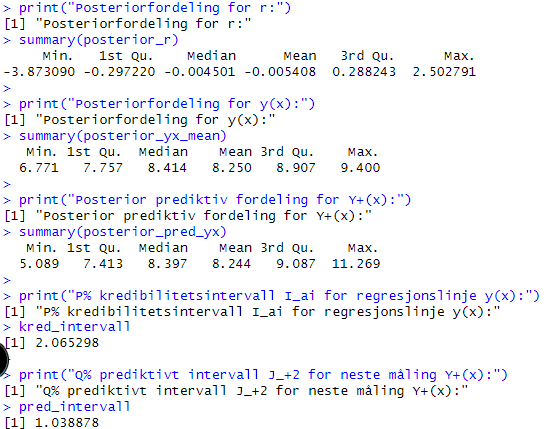
\includegraphics[width=0.8\textwidth]{1.png}
  \caption{(1)}
\end{figure}

\section{(15\%) kap. 17: oppgave 1.d}
\subsection{R kode}
\begin{verbatim}
  # Gitt data
  data <- cbind(c(0, 1, 2, 3), c(0, 2, 7, 5))
  
  # Gitte parametere
  alpha <- 0.1
  alpha_pred <- 0.05
  
  # utvalgsstatistikk
  n <- nrow(data)
  x_bar <- mean(data[, 1])
  y_bar <- mean(data[, 2])
  s_xx <- sum((data[, 1] - x_bar)^2)
  s_xy <- sum((data[, 1] - x_bar) * (data[, 2] - y_bar))
  
  # Posteriorfordeling for stigningstall a og skjæringspunkt b
  alpha_post <- n / 2
  beta_post <- 1 / (1 + alpha * s_xx)
  mu_post <- beta_post * alpha * sum(data[, 1] * data[, 2])
  tau_post <- alpha_post * beta_post
  b_post <- rnorm(10000, mean = mu_post, sd = sqrt(1 / tau_post))
  a_post <- rgamma(10000, shape = alpha_post, rate = beta_post)
  
  # Posterior prediktiv fordeling for Y+(x)
  posterior_pred_yx <- matrix(0, nrow = 10000, ncol = n)
  for (i in 1:10000) {
    posterior_pred_yx[i, ] <- rnorm(n, mean = a_post[i] * data[, 1] + b_post[i], sd = sqrt(1 / tau_post))
  }
  
  # P % kredibilitetsintervall I_ai for regresjonslinjen y(x)
  t_kritisk <- qt(1 - alpha / 2, df = n - 2)
  kredibilitetsintervall <- t_kritisk * sqrt((1 / n) + (s_xx / sum((data[, 1] - x_bar)^2)))
  
  # Q % prediktivt intervall J_+2 for neste måling Y+(x)
  z_kritisk <- qnorm(1 - alpha_pred / 2)
  prediktivt_intervall <- z_kritisk * sqrt((1 / n) + (s_xx / sum((data[, 1] - x_bar)^2)))
  
  # Resultater
  print("Posteriorfordeling for stigningstall a:")
  summary(a_post)
  
  print("Posteriorfordeling for skjæringspunkt b:")
  summary(b_post)
  
  print("Posterior prediktiv fordeling for Y+(x):")
  summary(posterior_pred_yx)
  
  print("P % kredibilitetsintervall I_ai for regresjonslinjen y(x):")
  kredibilitetsintervall
  
  print("Q % prediktivt intervall J_+2 for neste måling Y+(x):")
  prediktivt_intervall
  
    \end{verbatim}
SVAR:
\begin{figure}[H]
  \centering
  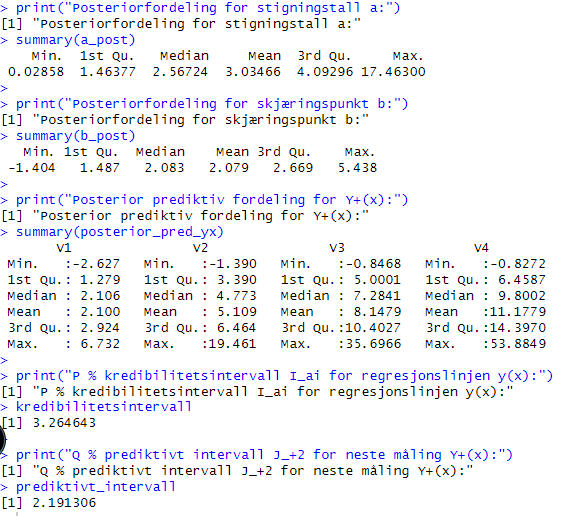
\includegraphics[width=0.8\textwidth]{2.png}
  \caption{(2)}
\end{figure}


\section{Terningdropp-oppgaven: (Totalt 50\%)}
\subsection{(5\%) Tegn et diagram med samtlige datapunkter, og legg på den lineære regresjonslinjen.}
\subsubsection{R kode}
\begin{verbatim}
      # Les inn data fra CSV-filen
      data <- read.csv('terningDropp.csv')
      
      # Utfør lineær regresjon
      fit <- lm(Lengde ~ Dropp, data=data)
      
      # Lag plot med datapunkter og regresjonslinje
      plot(data$Dropp, data$Lengde, xlab='Dropphøyde', ylab='Lengde', main='Terningdropp: Dropphøyde vs. Lengde')
      abline(fit, col='red')  
    \end{verbatim}
SVAR:
\begin{figure}[H]
  \centering
  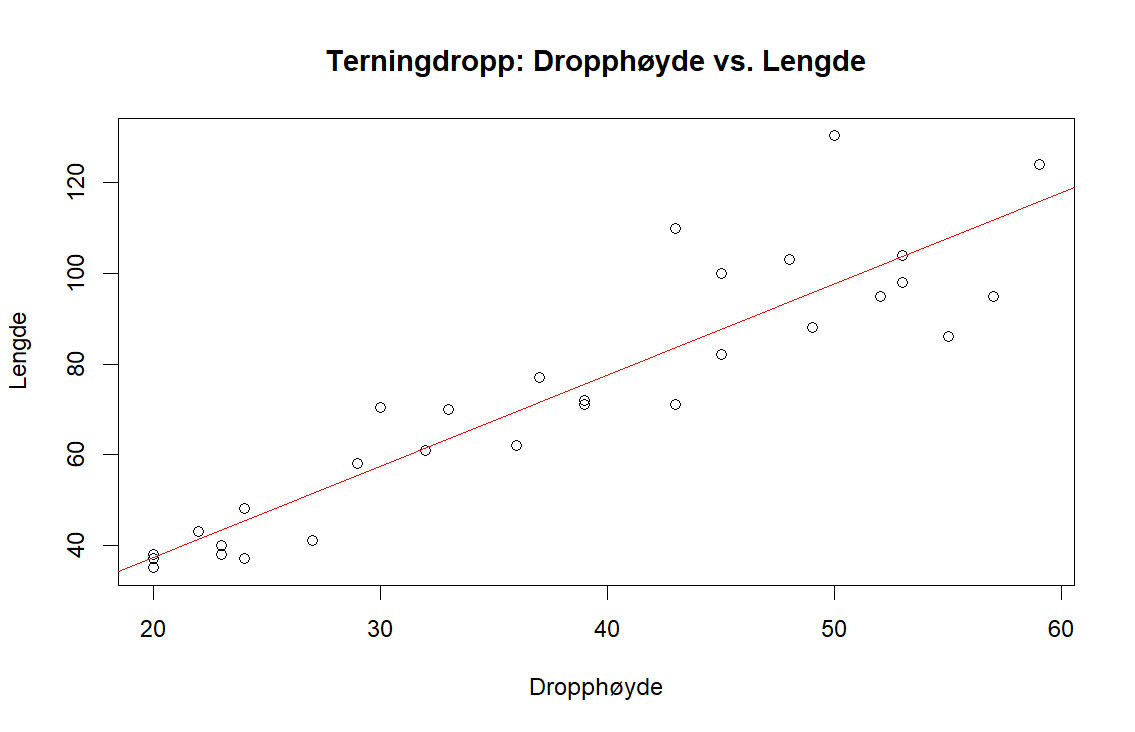
\includegraphics[width=0.8\textwidth]{3a.png}
  \caption{(3a)}
\end{figure}

\subsection{ $(15\%)$ Bruk nøytrale prior hyperparametre, og finn posterior og prediktive sannsynlighetsfordelinger, det vil si, sannsynlighetsfordelinger for $\tau$, $b$, $y(x)$ og $Y^+(x)$.}
\subsubsection{R kode}
\begin{verbatim}
  # Prior hyperparametre
  alpha <- 1
  beta <- 1
  
  # Likelihood hyperparametre
  mu0 <- 0
  sigma0 <- 1
  
  # Beregn posterior hyperparametre
  n <- length(data$Lengde)
  x_bar <- mean(data$Dropp)
  s_xx <- sum((data$Dropp - mean(data$Dropp))^2)
  
  alpha_post <- alpha + n/2
  beta_post <- beta + 1/2 * s_xx
  
   # Definer sannsynlighetsfordelingen for tau
  tau_values <- seq(0.001, 10, by = 0.01)
  prior_tau <- dgamma(tau_values, shape = alpha, scale = beta)
  
  # Plot sannsynlighetsfordelingen for tau
  plot(tau_values, prior_tau, type = "l", col = "blue", lwd = 2, xlab = "tau", ylab = "P(tau)",
       main = "Prior sannsynlighetsfordeling for tau (precision parameter)")
\end{verbatim}
SVAR:
\begin{figure}[H]
  \centering
  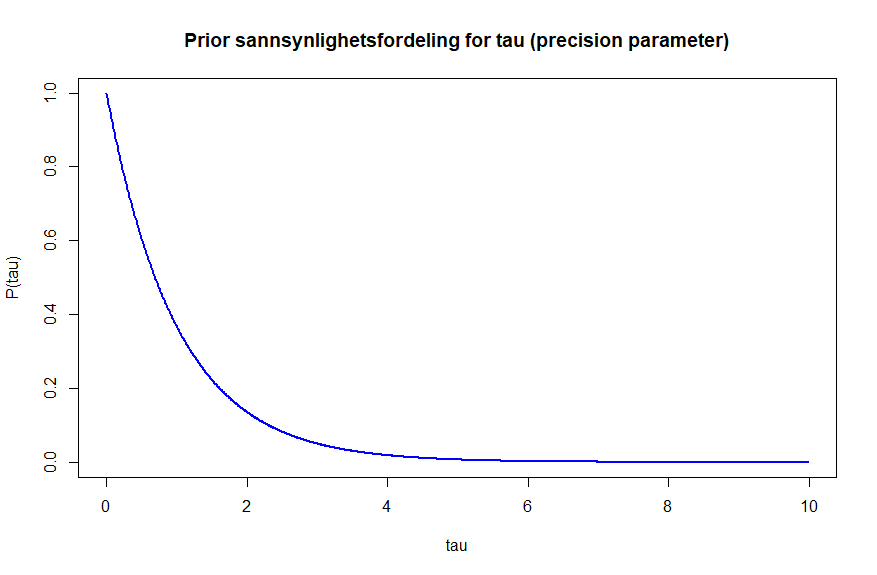
\includegraphics[width=0.8\textwidth]{3b-v2.png}
  \caption{(3b-v2)}
\end{figure}

\subsection{(5\%) Finn et 80\% kredibilitetsintervall (intervallestimat) for stigningstallet $b$.}
\subsubsection{R kode}
\begin{verbatim}
  # Bruk sannsynlighetsfordelingen fra oppgave 3b
  alpha_post <- alpha + n/2
  beta_post <- beta + 1/2 * s_xx
  
  # Generer posterior for tau (gamma-fordeling)
  posterior_tau <- rgamma(10000, shape = alpha_post, rate = beta_post)
  
  # resultater
  print(paste("Posterior for tau (precision parameter): Gamma(", alpha_post, ",", beta_post, ")"))
\end{verbatim}
SVAR:
\begin{figure}[H]
  \centering
  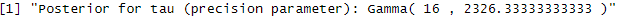
\includegraphics[width=0.8\textwidth]{3c-v2.png}
  \caption{(3c-v2)}
\end{figure}



\subsection{(5\%) Finn et 80\% kredibilitetsintervall (intervallestimat) for standardavviket $\sigma$. (Hint: Bruk verdiene fra $\tau$ og regn om ved å bruke at $\tau = \frac{1}{\sigma^2}$)}
\subsubsection{R kode}
\begin{verbatim}
  # Bruk sannsynlighetsfordelingen fra oppgave 3b
  lower_bound_sigma <- sqrt(1 / qgamma(alpha/2, shape = alpha_post, scale = 1/beta_post))
  upper_bound_sigma <- sqrt(1 / qgamma(1 - alpha/2, shape = alpha_post, scale = 1/beta_post))
  
  # Print resultatet
  print(paste("80% kredibilitetsintervall for standardavviket sigma: [", lower_bound_sigma, ",", upper_bound_sigma, "]"))
\end{verbatim}
SVAR:

\begin{figure}[H]
  \centering
  
\includegraphics[width=1\textwidth]{3d-v2.png}
  \caption{(3d-v2)}
\end{figure}

\subsection{(5\%) Finn et 80\% kredibilitetsintervall (intervallestimat) for $y(x)$.}
\subsubsection{R kode}
\begin{verbatim}
  # Prior hyperparametre
  alpha <- 1
  beta <- 1
  
  # Likelihood hyperparametre
  mu0 <- 0
  sigma0 <- 1
  
  # Beregn posterior hyperparametre
  n <- length(data$Lengde)
  x_bar <- mean(data$Dropp)
  s_xx <- sum((data$Dropp - mean(data$Dropp))^2)
  
  alpha_post <- alpha + n/2
  beta_post <- beta + 1/2 * s_xx
  
  # Generer posterior for tau (gamma-fordeling)
  posterior_tau <- rgamma(10000, shape = alpha_post, rate = beta_post)
  
  # Beregn prediktive fordelinger for tau
  pred_tau <- rgamma(10000, shape = alpha_post, rate = beta_post)
  pred_sigma <- 1 / sqrt(pred_tau)
  pred_b <- rnorm(10000, mu0, sigma0 * sqrt(1 / pred_tau))
  
  # Prediktiv fordeling for y(x)
  pred_yx <- pred_b * data$Dropp
  
  # Beregn 80% kredibilitetsintervall for y(x)
  lower_bound_yx <- quantile(pred_yx, 0.1)
  upper_bound_yx <- quantile(pred_yx, 0.9)
  
  print(paste("80% kredibilitetsintervall for y(x): [", lower_bound_yx, ",", upper_bound_yx, "]"))
\end{verbatim}
SVAR:
\begin{figure}[H]
  \centering
  
\includegraphics[width=1\textwidth]{3e-v2.png}
  \caption{(3e-v2)}
\end{figure}



\subsection{(5\%) 80\% intervallestimatet for $y(x)$ er funksjoner av $x$, og en kurve over, og en under regresjonslinjen. Plott disse kurvene inn sammen med regresjonslinjen.}
\subsubsection{R kode}
\begin{verbatim}
  # plusse på koden fra a
  # Plot datapunkter og regresjonslinje
  plot(data$Dropp, data$Lengde, xlab='Dropphøyde', ylab='Lengde', main='Terningdropp: Dropphøyde vs. Lengde')
  abline(fit, col='red')
  
  # Plot 80% kredibilitetsintervall for y(x)
  lines(data$Dropp, pred_mean + t_critical * sqrt(pred_var), col='blue')
  lines(data$Dropp, pred_mean - t_critical * sqrt(pred_var), col='blue')
  
  # Legg til en forklaring i plottet
  legend('topright', legend=c('Datapunkter', 'Regresjonslinje', '80% KI for y(x)'), col=c('black', 'red', 'blue'), lty=1)  
\end{verbatim}
SVAR:
\begin{figure}[H]
  \centering
  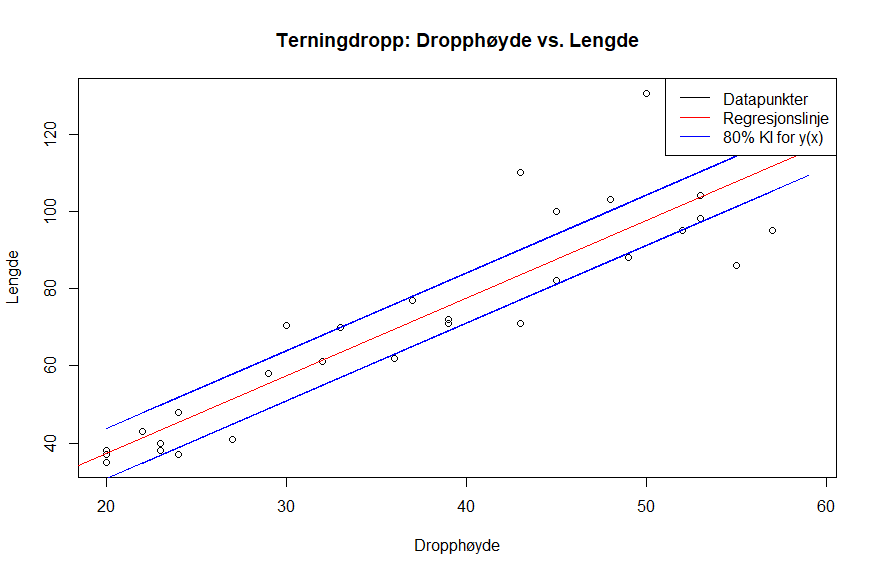
\includegraphics[width=1\textwidth]{3f.png}
  \caption{(3f)}
\end{figure}


\subsection{(5\%) Finn verdien $R^2 = \frac{SS_y - SS_e}{SS_y}$. Dette tallet forteller hvor stor del av variasjonen i $y$ som kan forklares av linja $y = a + bx$. For de av dere som bruker dataverktøy for å finne dette: angi hvordan dere fant det.}
\subsubsection{R kode}
\begin{verbatim}
  # Beregn R^2
  SS_y <- sum((data$Lengde - mean(data$Lengde))^2)
  SS_e <- sum(residuals(fit)^2)
  R_squared <- (SS_y - SS_e) / SS_y
  
  print(paste("Verdien av R^2:", R_squared)) 
\end{verbatim}
SVAR:
\begin{figure}[H]
  \centering
  
\includegraphics[width=1\textwidth]{3g.png}
  \caption{(3g)}
\end{figure}


\subsection{(5\%) Finn $R^2$ for regresjonen mellom $z$ (utfall på terningen) og $x$ (dropphøyde). Kommenter hva forskjellen mellom $R^2$ for $y$ og $R^2$ for $z$ sier oss.}
\subsubsection{R kode}
\begin{verbatim}
  # Utfør lineær regresjon for z vs. x
  fit_z <- lm(Verdi ~ Dropp, data=data)
  
  # Beregn R^2 for z
  SS_z <- sum((data$Verdi - mean(data$Verdi))^2)
  SS_e_z <- sum(residuals(fit_z)^2)
  R_squared_z <- (SS_z - SS_e_z) / SS_z
  
  print(paste("Verdien av R^2 for z:", R_squared_z))
  print("Forskjellen mellom R^2 for y og R^2 for z indikerer hvor mye av variasjonen i utfallet på terningen (z) og lengden (y) som forklares av modellen.")
  
\end{verbatim}
SVAR:
\begin{figure}[H]
  \centering
  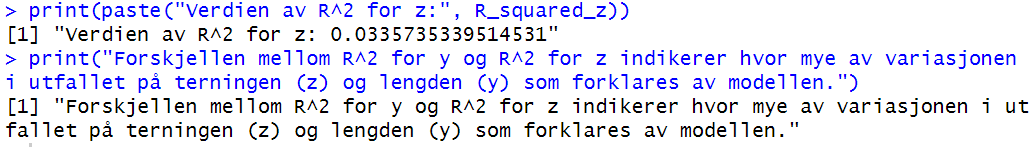
\includegraphics[width=1\textwidth]{3i.png}
  \caption{(3i)}
\end{figure}


\section{(Totalt 20\%) Følgende R-kode vil plukke ut et utvalg av observasjonene.}
\subsection{(5\%) Kjør 50 runder, og bruk $N = 15$. For hver runde, gjør oppgave 3a, men tegn regresjonslinjene sammen, i samme graf. Hva ser du?}
\subsection{(5\%) Kjør en runde med $N$ henholdsvis lik 5, 15, 50 og 200. For hver runde, gjør oppgavene 3c og 3d. Hva ser du?}
\subsection{(10\%) Kjør en runde med $N$ henholdsvis lik 5, 15, 50 og 200. For hver runde, gjør oppgaven 3f. Tegnes i hvert sitt diagram. Hva ser du?}

\newpage
\section*{Vedlegg}
\addcontentsline{toc}{section}{Vedlegg}
\subsection*{Vedlegg A}
\addcontentsline{toc}{subsection}{Vedlegg A}

\newpage
\begin{thebibliography}{9}

  \bibitem{referanse1}
  \url{https://tma4245.math.ntnu.no/viktige-diskrete-fordelinger/poissonprosess-og-poissonfordeling}
  \textit{NTNU}
\end{thebibliography}
\end{document}

